% standalone wrapper for a tikz picture
\documentclass[tikz,border=2pt]{standalone}
\usepackage{xcolor}
\usepackage{tikz}
\usetikzlibrary{shapes,arrows,positioning,shadows,patterns,arrows.meta,calc}
\definecolor{cwAlert}{RGB}{220,50,50}
\definecolor{cwFlow}{RGB}{50,120,220}
\definecolor{cwDecoy}{RGB}{120,180,50}
\definecolor{cwBorder}{RGB}{80,80,80}
\definecolor{ImperialBlue}{RGB}{0,62,116}
\definecolor{ImperialNavy}{RGB}{0,33,71}
\definecolor{ImperialLightBlue}{RGB}{155,203,235}
\begin{document}

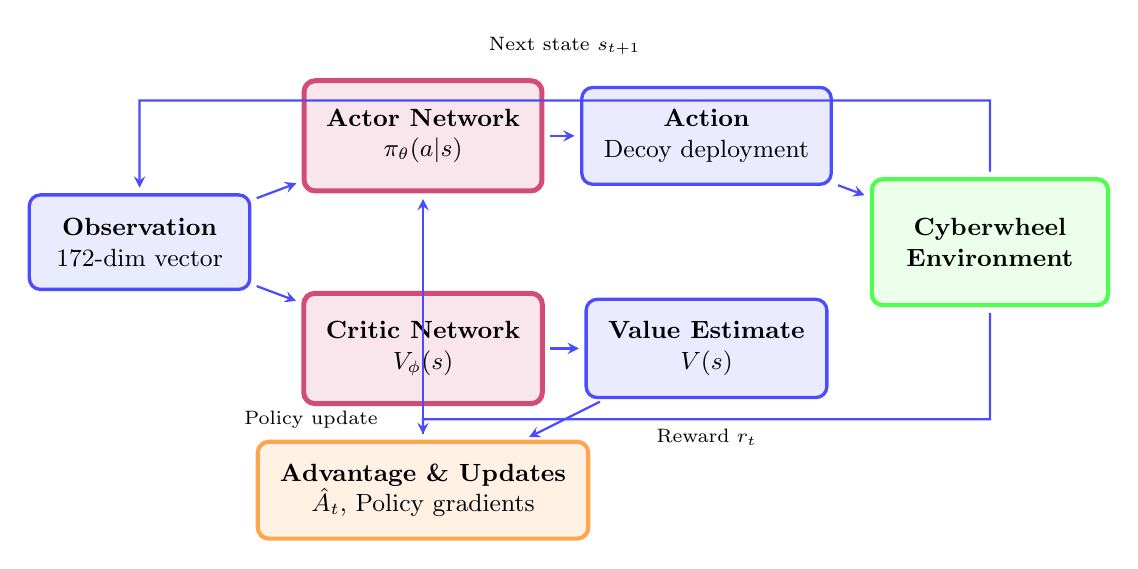
\begin{tikzpicture}[
    node distance=3cm,
    main/.style={draw=blue!70, rounded corners=4pt, fill=blue!8, 
                 inner sep=8pt, minimum width=2.8cm, minimum height=1.2cm, 
                 align=center, font=\small, line width=1.2pt},
    network/.style={draw=purple!70, rounded corners=4pt, fill=purple!10, 
                   inner sep=8pt, minimum width=2.8cm, minimum height=1.4cm, 
                   align=center, font=\small, line width=1.8pt},
    env/.style={draw=green!70, rounded corners=4pt, fill=green!8, 
               inner sep=8pt, minimum width=3cm, minimum height=1.6cm, 
               align=center, font=\small, line width=1.5pt},
    reward/.style={draw=orange!70, rounded corners=4pt, fill=orange!10, 
                   inner sep=8pt, minimum width=3.2cm, minimum height=1.2cm, 
                   align=center, font=\small, line width=1.5pt},
    flow/.style={-stealth, thick, blue!70, shorten >=2pt, shorten <=2pt},
    scale=0.9
]

% Left column: Input
\node[main] (obs) at (0,0) {
    \textbf{Observation}\\
    172-dim vector
};

% Center column: Networks
\node[network] (actor) at (4,1.5) {
    \textbf{Actor Network}\\
    $\pi_\theta(a|s)$
};

\node[network] (critic) at (4,-1.5) {
    \textbf{Critic Network}\\
    $V_\phi(s)$
};

% Right column: Outputs and Environment
\node[main] (action) at (8,1.5) {
    \textbf{Action}\\
    Decoy deployment
};

\node[main] (value) at (8,-1.5) {
    \textbf{Value Estimate}\\
    $V(s)$
};

\node[env] (environment) at (12,0) {
    \textbf{Cyberwheel}\\
    \textbf{Environment}
};

% Bottom: Learning components
\node[reward] (advantage) at (4,-3.5) {
    \textbf{Advantage \& Updates}\\
    $\hat{A}_t$, Policy gradients
};

% Forward flows (left to right, no crossing)
\draw[flow] (obs) -- (actor);
\draw[flow] (obs) -- (critic);
\draw[flow] (actor) -- (action);
\draw[flow] (critic) -- (value);
\draw[flow] (action) -- (environment);

% Feedback flows (right to left, separated levels)
\draw[flow] (environment) -- ++(0,2) -- ++(-12,0) -- (obs);
\node[above, font=\scriptsize] at (6,2.5) {Next state $s_{t+1}$};

\draw[flow] (environment) -- ++(0,-2.5) -- ++(-8,0) -- (advantage);
\node[below, font=\scriptsize] at (8,-2.5) {Reward $r_t$};

\draw[flow] (value) -- (advantage);

% Update flow (bottom to top, no crossing)
\draw[flow] (advantage) -- (actor);
\node[left, font=\scriptsize] at (3.5,-2.5) {Policy update};

\end{tikzpicture}
\end{document}
